\documentclass{beamer}
%\usepackage{fontspec}

\usetheme{Boadilla}
%\setmainfont{Latin Modern Sans}

%\includeonlyframes{current}

\usefonttheme{structurebold}
\usepackage{listings}
\usepackage{ragged2e}

\usepackage{pgf}
\usepackage{tikz}
\usepackage{alltt}
\usepackage[normalem]{ulem}
\usetikzlibrary{arrows}
\usetikzlibrary{automata}
\usetikzlibrary{shapes}
\usepackage{amsmath,amssymb}
\usepackage{rotating}
\usepackage{ulem}
\usepackage{listings}
\usepackage{enumerate}
\usepackage{tikz}
\tikzset{
  every overlay node/.style={
    draw=black,fill=white,rounded corners,anchor=north west,
  },
}
\def\tikzoverlay{%
   \tikz[baseline,overlay]\node[every overlay node]
}%

%\setbeamercovered{dynamic}
\setbeamertemplate{footline}[page number]{}
\setbeamertemplate{navigation symbols}{}
\usefonttheme{structurebold}

\title{Software Testing, Quality Assurance \& Maintenance---Lecture 23}
\author{Patrick Lam}
\date{March 13, 2019}

\colorlet{redshaded}{red!25!bg}
\colorlet{shaded}{black!25!bg}
\colorlet{shadedshaded}{black!10!bg}
\colorlet{blackshaded}{black!40!bg}

\colorlet{darkred}{red!80!black}
\colorlet{darkblue}{blue!80!black}
\colorlet{darkgreen}{green!80!black}

\newcommand{\rot}[1]{\rotatebox{90}{\mbox{#1}}}
\newcommand{\gray}[1]{\mbox{#1}}

\newenvironment{changemargin}[1]{% 
  \begin{list}{}{% 
    \setlength{\topsep}{0pt}% 
    \setlength{\leftmargin}{#1}% 
    \setlength{\rightmargin}{1em}
    \setlength{\listparindent}{\parindent}% 
    \setlength{\itemindent}{\parindent}% 
    \setlength{\parsep}{\parskip}% 
  }% 
  \item[]}{\end{list}}


\lstset{ %
language=C++,
basicstyle=\ttfamily,commentstyle=\scriptsize\itshape,showstringspaces=false,breaklines=true}

\begin{document}

\begin{frame}
  \titlepage
\end{frame}

\begin{frame}
\frametitle{Today}
\begin{changemargin}{2cm}
  Result Verification for Tests.\\[2em]
  Reference: Gerard Meszaros. \emph{xUnit Test Patterns: Refactoring Test Code}.
\end{changemargin}
\end{frame}

\begin{frame}
  \frametitle{Goal}

  \Large
  \begin{changemargin}{2cm}
    Good tests are \emph{self-checking}:\\[1em]
    no errors, no failures = successful test.
  \end{changemargin}

  \begin{center}
    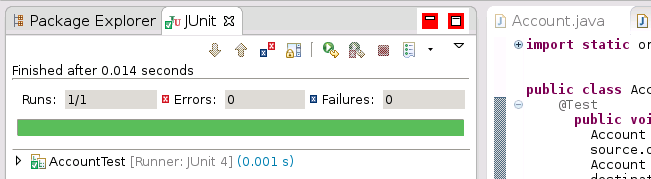
\includegraphics[width=.6\textwidth]{L23/pass}
  \end{center}
  
\end{frame}

\begin{frame}
  \frametitle{Why Self-Checking Tests?}

  \Large
  \begin{changemargin}{2cm}
    Tests automatically report status.\\[1em]
    Enables ``keep the bar green''\\
    coding style.\\[1em]
    Worry less about introducing bugs.\\[1em]
    Plus: Tests help document system specs.
  \end{changemargin}
\end{frame}

\begin{frame}
  \frametitle{Today's Plan}

  \Large
  \begin{changemargin}{1cm}
    HOWTO make your tests self-checking.
  \end{changemargin}
\end{frame}

\begin{frame}
  \Large
  \begin{changemargin}{2cm}
    ``Isn't it just calling asserts?''\\[1em]
\only<2>{    \hspace*{4cm} [sadly, no.]}
  \end{changemargin}
\end{frame}

\begin{frame}
  \Large
  \begin{changemargin}{2cm}
    Two questions about asserts:
    \begin{enumerate}
    \item Q: what for?\\
      A: check method call results\\[1em]
    \item Q: where?\\
      A: usually after calling SUT \\ ~~~~(System Under Test)
    \end{enumerate}
  \end{changemargin}
\end{frame}

\begin{frame}
  \frametitle{Counter Example}

  \begin{changemargin}{2cm}
    \lstinputlisting{L23/Counter.java}
  \end{changemargin}
\end{frame}

\begin{frame}
  \frametitle{Counter Test}

  \begin{changemargin}{2cm}
    \lstinputlisting{L23/CounterTest.java}
  \end{changemargin}
\end{frame}

\begin{frame}
  \frametitle{State or Behaviour?}

  \begin{changemargin}{2cm}
    Was Counter Test verifying state or behaviour?
  \end{changemargin}
\end{frame}

\begin{frame}
  \frametitle{State vs Behaviour}

  \large
  \begin{changemargin}{2cm}
    {\bf State:} e.g. object field values.\\
    \hspace*{1.5cm}
    Call accessor methods to verify.\\[1em]
    {\bf Behaviour:} which calls SUT makes.\\
    \hspace*{1.5cm} Insert observation points, \\ \hspace*{1.5cm} monitor interactions.
  \end{changemargin}
\end{frame}

\begin{frame}
  \frametitle{Flight example}

  \small
    \lstinputlisting{L23/flight.java}
\end{frame}

\begin{frame}
  \frametitle{Flight example: state verification}

  \small
    \lstinputlisting{L23/flight_extended_state_spec.java}
\end{frame}

\begin{frame}
  \frametitle{What Is State Verification?}

  \Large
  \begin{changemargin}{2cm}
    \begin{enumerate}
    \item Exercise SUT.
    \item Verify state \& check return values.
    \end{enumerate}

    ~\\[1em]
    Inspect only outputs; \\ \hspace*{1cm} only call methods from SUT.\\[1em]
    Do not instrument SUT.\\[1em]
    Do not check interactions.
  \end{changemargin}
\end{frame}

\begin{frame}
  \frametitle{Implementing State Verification}

  \Large
  \begin{changemargin}{2cm}
    Two options:
    \begin{enumerate}
    \item procedural (bunch of asserts); or,
    \item via expected objects (stay tuned).
    \end{enumerate}
  \end{changemargin}
\end{frame}

\begin{frame}
  \frametitle{Flight Example: discussing state verification}

  \large
  \begin{changemargin}{2cm}
    We do check that the flight got removed.\\
    We don't check that the removal got logged.\\[1em]
    Hard to check state and observe logging.\\[1em]
    Solution: Spy on SUT behaviour.
  \end{changemargin}
\end{frame}


\begin{frame}
  \frametitle{Flight example: procedural behaviour verification}

  \small
    \lstinputlisting{L23/flight_pbv.java}
\end{frame}

\begin{frame}
  \frametitle{Alternative: Expected Behaviour Specification}
  \Large
  \begin{changemargin}{2cm}
    Use a mock object framework (e.g. JMock)\\
    to define expected behaviour.\\[1em]

    Observe calls to the logger, \\
    make sure right calls happen.
  \end{changemargin}
\end{frame}

\begin{frame}
  \frametitle{Kinds of Assertions}
  \large
  \begin{changemargin}{2cm}
    Three built-in choices:
    \begin{enumerate}
    \item assertTrue(aBooleanExpression)
    \item assertEquals(expected, actual)
    \item assertEquals(expected, actual, tolerance)
    \end{enumerate}
    ~\\[1em]
    note: {\tt assertTrue} can give \\
    hard-to-diagnose error messages \\
    (must try harder when using).
  \end{changemargin}
\end{frame}

\begin{frame}
  \frametitle{Using Assertions}
  \large
  \begin{changemargin}{2cm}
    Assertions are good:
    \begin{itemize}
    \item to check all things that should be true\\
      \begin{changemargin}{1cm}
        (more = better)
      \end{changemargin}
    \item to serve as documentation:
      \begin{changemargin}{1cm}
        when system in state $S_1$,\\
        and I do $X$,\\
        assert that the result should be $R$, and\\
        that system should be in $S_2$.
      \end{changemargin}
    \item to allow failure diagnosis\\
            \begin{changemargin}{1cm}
              (include assertion messages!)
            \end{changemargin}
    \end{itemize}
  \end{changemargin}
\end{frame}

\begin{frame}
  \frametitle{Not Using Assertions}
  \Large
  \begin{changemargin}{2cm}
    Can also do external result verification:\\[1em]
    Write output to files, diff (or custom diff)
    expected and actual output.\\[1em]
    Twist: expected result then not visible when looking at test.\\[1em]
    (What's a good workaround?)
  \end{changemargin}
\end{frame}

\begin{frame}
  \frametitle{Verifying Behaviour}
  \Large
  \begin{changemargin}{2cm}
    Observe actions (calls) of the SUT.
    \begin{itemize}
    \item procedural behaviour verification; or,\\
      (challenge: recording \& verifying behaviour)\\[.5em]
    \item via expected behaviour specification.\\
      (also captures outbound calls of SUT)
    \end{itemize}
  \end{changemargin}
\end{frame}


\begin{frame}
  \frametitle{So far\ldots}
  \Large
  \begin{changemargin}{2cm}
    Seen the basics of result verification.\\[1em]
    Next: how to improve your tests!
  \end{changemargin}
\end{frame}

\begin{frame}
  \frametitle{Reducing Test Code Duplication}
  \Large
  \begin{changemargin}{2cm}
    Usual cause: copy-pasta.\\[1em]

    Mitigating duplication in result verification:
    \begin{itemize}
    \item Expected Objects
    \item Custom Assertions
    \item Verification Methods
    \end{itemize}
  \end{changemargin}
\end{frame}

\begin{frame}
  \frametitle{Duplication-Prone Test Method}
  \begin{changemargin}{1.5cm}
    \large
    One might expect many test methods like this one.
  \end{changemargin}
  \small
    \lstinputlisting{L23/testInvoice.java}
\end{frame}

\begin{frame}
  \frametitle{Using an Expected Object}
  \begin{changemargin}{1.5cm}
    \large
    We can compare objects instead:
  \end{changemargin}
  \small
  \begin{changemargin}{1cm}
    \lstinputlisting{L23/testInvoice-equality.java}
  \end{changemargin}
  \begin{changemargin}{1.5cm}
    \large
    Need:
    \begin{itemize}
    \item a way to create the Expected Object;
    \item a suitable {\tt equals()} method.
    \end{itemize}
  \end{changemargin}
\end{frame}

\begin{frame}
  \frametitle{Potential Issues}
  \Large
  \begin{changemargin}{1.5cm}
    Perhaps we:
    \begin{itemize}
    \item need special {\tt equals()} method, \\
      e.g. to compare subset of fields; or,
    \item may only have {\tt equals()} that checks identity; or,
    \item can't create desired expected object.
    \end{itemize}
    ~\\
    Solutions:
    \begin{itemize}
    \item create custom assertion; or,
    \item provide special {\tt equals()} on expected object.
    \end{itemize}
  \end{changemargin}
\end{frame}

\begin{frame}
  \frametitle{Custom Assertions Example}
  \begin{changemargin}{.5cm}
    \small
    \lstinputlisting{L23/testInvoice-custom-assertion.java}
  \end{changemargin}

  \begin{changemargin}{2cm}
    \Large
    Pick a good, declarative name.\\
    Obtain by refactoring, \\ \hspace*{2cm} using usual techniques.
  \end{changemargin}
\end{frame}

\begin{frame}
  \frametitle{Benefits of Custom Assertions}

  \begin{changemargin}{2cm}
    \Large
    \begin{itemize}
      \item Hide irrelevant detail.
        \item Label actions with a good name.
        \item Are themselves testable.
    \end{itemize}
  \end{changemargin}
\end{frame}

\begin{frame}
  \frametitle{Variant: Outcome-describing Verification Method}
  \begin{changemargin}{.5cm}
    \small
    \lstinputlisting{L23/testInvoice-verification-method.java}
  \end{changemargin}

  \begin{changemargin}{2cm}
    Differences: a verification method
    \begin{itemize}
    \item also interacts with SUT;
      \item may have arbitrary parameters.
    \end{itemize}
  \end{changemargin}
\end{frame}

\begin{frame}
  \frametitle{Going Further: Parameterized, Data-Driven Tests}
  \begin{changemargin}{2cm}
    \Large
    While we're at it,\\
    we can have entire tests \\
    that differ only in input data.\\[1em]
    Concrete tests invoke  parametrized tests.
  \end{changemargin}
\end{frame}

\begin{frame}[fragile]
  \frametitle{Avoiding Logic in Tests}
  \begin{changemargin}{2cm}
    Problem: tests are untestable.\\
    Including ifs and loops in tests = danger!\\
  \end{changemargin}
  {\small
    \begin{lstlisting}
  // BAD
  List lineItems = invoice.getLineItems();
  if (lineItems.size() == 1) {
    // ...
  } else {
    fail("Invoice should have exactly 1 line item");
  }
    \end{lstlisting}
    }
  \begin{changemargin}{2cm}
  Instead, do this:
  \end{changemargin}
      {\small
    \begin{lstlisting}
  // GOOD
  List lineItems = invoice.getLineItems();
  // (guard assertion:)
  assertEquals("number of items", lineItems.size(), 1);
  // ... proceed as before
    \end{lstlisting}
    }
  \begin{changemargin}{2cm}
    The guard keeps you out of trouble.
  \end{changemargin}
\end{frame}

\begin{frame}
  \frametitle{Loops}
  \Large
  \begin{changemargin}{2cm}
    Don't put loops directly in tests.\\[1em]
    Use a well-named, testable \\Test Utility Method instead.
  \end{changemargin}
\end{frame}

\begin{frame}
  \frametitle{Summary}
  \Large
  \begin{changemargin}{1cm}
    Practical techniques for writing tests.\\[1em]

    Today's focus: result verification.
    \begin{itemize}
    \item state verification
    \item behaviour verification
    \end{itemize}~\\

    Also, techniques for improving your tests.
    \begin{itemize}
    \item reducing duplication
    \item simplifying tests
    \end{itemize}

  \end{changemargin}
\end{frame}

\end{document}
